\section{Forschungsfragen}

\begin{figure}[htb!]
    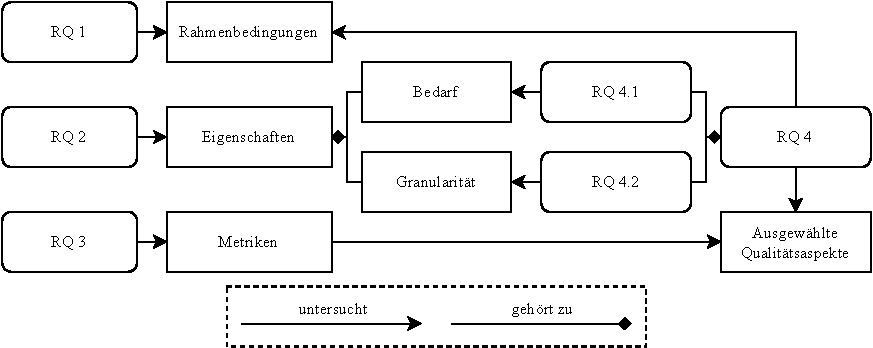
\includegraphics[width=\textwidth]{contents/03_research_design/res/research_questions_overview.pdf}
    \caption{Zusammenhänge der Forschungsfragen}
    \label{fig:research_questions_overview}
\end{figure}

Aus dem Forschungsziel wurden fünf Forschungsfragen (\textit{Research Questions, RQ}) abgeleitet, welche die Richtung der Arbeit fein granularer definieren. Jede Forschungsfrage behandelt entweder einen konkreten Betrachtungsgegenstand von Erklärbarkeit oder den Zusammenhang der einzelnen Aspekte. Wie die einzelnen Forschungsfragen zusammenhängen, ist in \autoref{fig:research_questions_overview} dargestellt.

\smallskip

\noindent\fbox{
    \parbox{0.964\textwidth}{
        \smallskip
        \textbf{RQ1} Welche Rahmenbedingungen und Ziele haben einen Einfluss auf die Anforderungen für Erklärungen?
        \smallskip
    }
}

\smallskip

Erklärbare Systeme können sehr verschiedene Ausprägungen haben (z.B. Empfehlungssysteme \cite{kunkel_let_2019} oder autonome Fahrzeuge \cite{wiegand2019drive}). Auch werden je nach Anwendungsgebiet verschiedene Anforderungen an die Systeme gestellt oder es gibt zusätzlich geltende, äußere Bedingungen \cite{chazette_knowledge_nodate}.

Die Untersuchung dieser Aspekte auf die Einflüsse auf die benötigten Erklärungen bzw. Erklärbarkeit im Allgemeinen geschieht als Antwort auf diese Frage. Dabei sollen Rahmenbedingungen ausgearbeitet werden, welche für Anforderungen an Erklärungen relevant sind. Auch mögliche Ziele für Erklärungen soll die Antwort auf diese Forschungsfrage bieten. 

\smallskip

\noindent\fbox{
    \parbox{0.964\textwidth}{
        \smallskip
        \textbf{RQ2} Welche Eigenschaften von Erklärungen haben einen Einfluss auf die externe Qualität eines erklärbaren Systems?
        \smallskip
    }
}

\smallskip

Es existieren bereits verschiedene Frameworks, die für bestimmte Anwendungsbereiche die Gestaltungsmöglichkeiten für Erklärungen zusammenfassen \cite{nunes_systematic_2017}. Vor allem im Bereich der Künstlichen Intelligenz gibt es zahlreiche Arbeiten, welche einen solchen Überblick geben, um automatisch Erklärungen für komplexe Algorithmen zu generieren \cite{sokol_explainability_2020, mahoney2019framework}.

Um der Forderung nach einem stärkeren Fokus auf den Menschen bei der Betrachtung von Erklärbarkeit nachzukommen \cite{ehsan_operationalizing_2021}, stellt diese Forschungsfrage die externen Qualitätsaspekte \cite{international2011iso} in den Mittelpunkt. Hierbei werden externe Qualitätsaspekte mit einbezogen, durch welche die Qualität von Erklärungen bestimmt werden kann. Außerdem werden im Rahmen dieser Frage unter anderem die Gestaltungsmöglichkeiten für den Bedarf an Erklärungen und deren Granularität betrachtet, die Entwicklern oder Designern bei der Konzeption von Erklärungen zur Verfügung stehen. 

% Folglich ist die Antwort auf diese Frage eine zentrale Grundlage für den Leitfaden, dessen Entwicklung ein Ziel dieser Arbeit ist.

\smallskip

\noindent\fbox{
    \parbox{0.964\textwidth}{
        \smallskip
        \textbf{RQ3} Auf welche Art und Weise kann evaluiert werden, ob die in ein erklärbares System integrierten Erklärungen das Ziel der Integration bezogen auf externe Qualitätsaspekte erfüllt haben?
        \smallskip
    }
}

\smallskip

Erklärbarkeit ist eine NFR, welche von vielen Faktoren abhängt und diese auch beeinflusst \cite{chazette_knowledge_nodate}. Die Integration von Erklärungen hat in der Regel Effekte auf mehrere andere Qualitätsaspekte. Diese Effekte können sowohl positiv als auch negativ sein. Durch die Integration von Erklärungen ist es unter anderem möglich, dass die \textit{Usability} des Systems verschlechtert wird, wenn sie nicht explizit mitgedacht wird \cite{sokol_explainability_2020}. Folglich stellt das Messen der Qualität von Erklärungen aufgrund der vielfältigen Effekte eine Herausforderung dar. Des Weiteren muss bei der Evaluation beachtet werden, dass viele der durch Erklärbarkeit beeinflussten NFRs vorwiegend subjektiv von Software-Nutzern wahrgenommen werden und somit nur wenige objektive Metriken einsetzbar sind \cite{sokol_explainability_2020}.

In der Literatur wurden bereits Erklärungen anhand verschiedener Metriken analysiert \cite{wiegand2019drive,briand1995goal}. Es fehlt allerdings ein Überblick, welche Metriken zum Messen und zur Bewertung der Qualität von Erklärungen geeignet und erprobt sind. Folglich ist das Ziel bei der Beantwortung dieser offenen Frage, die bereits zur Evaluation von Erklärungen genutzten Metriken zusammenzutragen.

\smallskip

\noindent\fbox{
    \parbox{0.964\textwidth}{
        \smallskip
        \textbf{RQ4.1} Welchen Einfluss hat der Bedarf von Erklärungen auf die externe Qualität eines erklärbaren Systems unter bestimmten Rahmenbedingungen?

        \smallskip

        \textbf{RQ4.2} Welchen Einfluss hat die Granularität von Erklärungen auf die externe Qualität eines erklärbaren Systems unter bestimmten Rahmenbedingungen?
        \smallskip
    }
}

\smallskip

In den ersten drei Forschungsfragen wurden verschiedene Aspekte von Erklärbarkeit behandelt, die wichtig sind, um darauf basierend Erklärungen in ein System zu integrieren. Allerdings werden durch die Antworten auf die Fragen keine Empfehlungen für die richtige Auswahl der Aspekte gegeben. Diese Aufgabe soll durch die Antwort auf diese letzten beiden Fragen unterstützt werden.

Die Einflüsse, nach denen RQ4.1 fragt, sollen bei der Einschätzung helfen, ob und wenn ja, an welchen Stellen, ein System Erklärungen benötigt. Dies soll Entwicklern und Designern dabei helfen, die Frage nach dem Bedarf für Erklärungen Anwendungsfall-übergreifend zu beantworten. Für Navigationsanwendungen haben dies beispielsweise \citeauthor{chazette_end-users_nodate} sowie \citeauthor{wang_integration_2020} bereits getan \cite{chazette_end-users_nodate,wang_integration_2020}.

Wenn eben dieser Bedarf besteht, muss anschließend die Ausgestaltung dieser Erklärung betrachtet werden. Welche bereits untersuchten Einflüsse in Bezug auf diese Granularität von Erklärungen bestehen, soll die Antwort auf die Frage RQ4.2 beantworten.

Folglich stellen die Forschungsfragen RQ4.1 und RQ4.2 die Schnittstelle zwischen den ersten drei Forschungsfragen dar.